\documentclass[letterpaper, 10 pt, conference]{ieeeconf}

\IEEEoverridecommandlockouts
\overrideIEEEmargins 

\usepackage{graphicx}      % include this line if your document contains figures
\usepackage{amsmath,amssymb}
\usepackage{url}
\usepackage{diffcoeff}
\usepackage{bm}
\usepackage{cite}
\usepackage{subfig}
\usepackage{diffcoeff}
\usepackage{mathrsfs}
\usepackage{tikz}
\usetikzlibrary{shapes,arrows,positioning,calc}

\usepackage[bookmarks=false]{hyperref}
\usepackage{multirow}

\newtheorem{theorem}{Theorem}
\newtheorem{remark}{Remark}
\newtheorem{proposition}{Proposition}


\DeclareMathOperator*{\argmax}{arg\,max}
\DeclareMathOperator*{\argmin}{arg\,min}
\DeclareMathOperator{\Tr}{Tr}

\def\onedot{$\mathsurround0pt\ldotp$}
\def\cddot{% two dots stacked vertically
	\mathbin{\vcenter{\baselineskip.67ex
			\hbox{\onedot}\hbox{\onedot}}%
}}

\makeatletter \renewcommand\d[1]{\ensuremath{%
		\;\mathrm{d}#1\@ifnextchar\d{\!}{}}}
\makeatother

\title{\LARGE \bf
	Control by interconnection of the Kirchhoff plate
	within the port-Hamiltonian framework*	
}


\author{Andrea Brugnoli$^{1}$, Daniel Alazard$^{1}$, Val\'erie Pommier-Budinger$^{1}$ and Denis Matignon$^{1}$% <-this % stops a space
	\thanks{*This work is supported by the project ANR-16-CE92-0028,
		entitled {\em Interconnected Infinite-Dimensional systems for Heterogeneous
			Media}, INFIDHEM, financed by the French National Research Agency (ANR) and the Deutsche Forschungsgemeinschaft (DFG). Further information is available at { \url{https://websites.isae-supaero.fr/infidhem/the-project}}.}% <-this % stops a space
	\thanks{$^{1}$Andrea Brugnoli, Daniel Alazard, Val\'erie Pommier-Budinger and Denis Matignon are with ISAE-SUPAERO, Universit\'e de Toulouse, France,
		10 Avenue Edouard Belin, BP-54032, 31055 Toulouse Cedex 4
		{\tt\small \{Andrea.Brugnoli, Daniel.Alazard, Valerie.Budinger, Denis.Matignon\}@isae.fr} }
}

\graphicspath{{./Figures/}, {./Figures/DampingInjection/}, {./Figures/InterconnectionRod/}}

\begin{document}


\maketitle
\thispagestyle{empty}
\pagestyle{empty}

% make the title area
\maketitle

% As a general rule, do not put math, special symbols or citations
% in the abstract
\begin{abstract}
	The Kirchhoff plate model is detailed by using a tensorial port-Hamiltonian (pH) formulation. A structure-preserving discretization of this model is then achieved by using the partitioned finite element (PFEM). This methodology easily accounts for the boundary variables and the finite-dimensional system can be interconnected to the surrounding environment in a simple and structured manner. The algebraic constraints to be considered are deduced from the boundary conditions, that may be homogeneous or defined by an interconnection with another pH system. \\
	The versatility of the proposed approach is assessed by means of numerical simulations. A first illustration considers a rectangular plate clamped on one side and interconnected to a rigid rod welded to the opposite side. A second example exploits the collocated output feature of pH systems to perform damping injection in a plate undergoing an external forcing. A stability proof is obtained by the application of the LaSalle's invariance principle.
\end{abstract}

% no keywords




% For peer review papers, you can put extra information on the cover
% page as needed:
% \ifCLASSOPTIONpeerreview
% \begin{center} \bfseries EDICS Category: 3-BBND \end{center}
% \fi
%
% For peerreview papers, this IEEEtran command inserts a page break and
% creates the second title. It will be ignored for other modes.
\IEEEpeerreviewmaketitle



\section{Introduction}
The port-Hamiltonian (pH) framework has proved to be a powerful framework for modeling and control of multi-physics system \cite{bookPHs}. During the last years distributed systems, i.e. systems ruled by partial differential equations (PDEs) have attracted a lot of interest \cite{BookZwart}. The modularity property of the pH paradigm is particularly appealing as it provides a structured and coherent way to build complex system. Infinite- and finite- dimensional \cite{ShaftIntInfinite, CerveraIntFinite} pH systems can be connected together giving rise to another pH system. \\

In order to simulate and control such systems, a finite-dimensional representation of the distributed system has to be found and it is convenient to use a discretization procedure that preserves the port-Hamiltonian nature and uses standard numerical libraries. The first attempt to perform a structure-preserving discretization dates back to \cite{Golo}, where the authors proposed a mixed finite element spatial discretization for 1D hyperbolic system. Pseudo-spectral methods were studied in \cite{moulla:hal-01625008}. The prototypical example of hyperbolic systems of two conservation laws was discretized by a weak formulation in \cite{WeakForm_Kot}, leading to a Galerkin numerical approximations. A drawback of these methods is that they require specific implementations and cannot be easily related to standard numerical methods. An extension of the Mixed finite element method to pH system was proposed in \cite{CardosoRibeiro2018}. The main point of this methodology is that the integration by parts is performed so as to preserve the symplectic structure. Several choices of the boundary control are possible, hence this method is referred to as the partitioned finite element method (PFEM). If mixed boundary conditions have to be considered the discretized system is an algebraic differential one (pHDAEs), which can be analyzed by referring to \cite{beattie2018linear,vanderSchaft2013}. \\

In this paper the Kirchhoff plate model is presented in a pH fashion. Another classical model, the Mindlin plate, has already been enriched with a suitable Stokes-Dirac structure in \cite{MacchelliMindlin}. The formalism is here extended by employing  tensorial calculus in order to clearly identify the skew-symmetric nature of the differential operator. PFEM discretization is then used to obtain a finite-dimensional system. Numerical applications are then carried out using the Firedrake platform \cite{firedrake}. An interconnection along the boundary is presented to model a cantilever plate welded to a rigid bar. This serves just as an example as the methodology may be employed to construct complex systems starting from their basic components. A control application by damping injection follows. The plate is interconnected along part of the boundary with a dissipative system. The LaSalle's principle guarantees that the system will tend to the equilibrium point, i.e. the undeformed configuration. \\

Section \ref{sec:KirchhPH} describes the Kirchhoff Plate model in strong form as a port-Hamiltonian system . In Section \ref{sec:SP_discr} the structure-preserving discretization obtained by using PFEM  is detailed. The discretized system and the associated finite elements are given in \ref{subsec:finPHs}. Section \ref{sec:Int} provides a structured way to interconnect an infinite-dimensional system with a finite-dimensional one. The damping injection control methodology is briefly discussed in Section \ref{sec:Damp}. 

\section{pH formulation of the Kirchoff plate}
\label{sec:KirchhPH}

In this section the classical formulation of the Kirchhoff plate and the tensorial pH one are described. 

\subsection{Notations}
First, the differential operators needed in the following are recalled. For a scalar field $u: \mathbb{R}^d \rightarrow \mathbb{R}$ the gradient is defined as 
\begin{equation*}
\mathrm{grad}(u) =  \nabla u := \begin{pmatrix}
\partial_{x_1} u \dots \partial_{x_d} u \\
\end{pmatrix}^T.
\end{equation*}
For a vector field $\bm{v}: \mathbb{R}^d \rightarrow \mathbb{R}^d$ the symmetric part of the gradient operator $\mathrm{Grad}$ (i. e. the deformation gradient in continuum mechanics) is given by
\begin{equation*}
\mathrm{Grad}(\bm{v}) := \frac{1}{2} \left(\nabla \bm{v} + \nabla^T \bm{v} \right).
\end{equation*}
The Hessian operator of $u$ is then computed as follows
\begin{equation*}
\mathrm{Hess}(u) = \mathrm{Grad}(\mathrm{grad}(u)),
\end{equation*}
For a tensor field $\bm{U}: \mathbb{R}^d \rightarrow \mathbb{R}^{d \times d}$, with elements $u_{ij}$, the divergence is a vector, defined column-wise as
\begin{equation*}
\mathrm{Div}(\bm U) = \nabla \cdot \bm{U} := \left( \sum_{i = 1}^d \partial_{x_i} u_{ij} \right)_{j = 1, \dots, d}.
\end{equation*}
The double divergence of a tensor field $\bm{U}$ is then a scalar field defined as
\begin{equation*}
\mathrm{div}(\mathrm{Div}(\bm U)):= \sum_{i, j = 1}^d \partial_{x_i} \partial_{x_j} u_{ij} \, .
\end{equation*}
The geometrical dimension of interest in this paper is $d=2$. In the following vectors (tensor) fields and numerical vectors (matrices) will be denote by a lower (upper) case bold letter. It will be clear from the context which mathematical objects is being considered. Furthermore, $\mathbb{S}$ denotes the space of symmetric $d \times d$ tensors (matrices).
\subsection{Kirchhoff Model for Thin Plates}
\label{subsec:classMin}
The Kirchhoff Model is a generalization to the 2D case of the Euler-Bernoulli beam model and accounts for the shear deformation. Given an open and connected set $\Omega \in \mathbb{R}^2$, the classical equations for this model \cite{timoshenko1959theory} are 
\begin{equation}
\displaystyle \rho h \diffp[2]{w}{t} = -\mathrm{div}(\mathrm{Div}(\bm{M})), \\
\end{equation}
where $\rho$ is the material density, $h$ is the plate thickness, the scalar $w$ is the vertical displacement and $\bm{M}$ is the symmetric momenta tensor.  This tensor is related to the symmetric curvatures tensor $\bm{K}$ by the bending rigidity tensor, so that $\bm{M}_{ij} = \bm{D}_{ijkl} \bm{K}_{kl}$. The curvature tensor is defined as
\begin{equation*}
\bm{K} := \mathrm{Grad}(\mathrm{grad}(w)).
\end{equation*}
For an homogeneous isotropic material the components of $\bm{M}, \bm{K} \in \mathbb{S}$ are related by the relations ($x$ denotes index 1, $y$ index~2)
\begin{equation*}
\begin{aligned}
m_{xx} &= D\left(\kappa_{xx} + \nu \kappa_{yy}\right),\\
m_{yy} &= D\left(\kappa_{yy} + \nu \kappa_{xx}\right),\\
m_{xy} &= D(1 - \nu) \kappa_{xy}, \\
\end{aligned}
\end{equation*}
with $\nu$ the Poisson's ratio, $D$ the bending modulus. The kinetic and potential energy densities $\mathcal{K}$ and $\mathcal{U}$ read
\begin{equation}
\mathcal{K} =  \frac{1}{2}\rho h \left(\diffp{w}{t} \right)^2, \quad
\mathcal{U} = \frac{1}{2} \bm{M} \cddot \bm{K},
\end{equation} 
where $\bm{M} \cddot \bm{K} := \sum_{i,j} m_{ij} \kappa_{ij}$ is the tensor contraction. The Hamiltonian  is easily written as
\begin{equation} 
H = \int_{\Omega} \left( \mathcal{K} + \mathcal{U} \right)   \d\Omega. 
\end{equation}

\subsection{Tensorial Port-Hamiltonian formulation}
In order to rewrite the system as a port-Hamiltonian one, the energy variables have to be selected first. This  choice is analogous to that of the pH Euler-Bernoulli beam  model \cite{BrugnoliKir}, but with the complication that here the energy variables are of scalar and tensorial nature:
\begin{equation}
\begin{aligned}
\alpha_w &= \rho h \diffp{w}{t}, \quad &\text{Linear momentum}, \\
\bm{A}_{\kappa} &= \bm{K}, \quad &\text{Curvature tensor}.\\
\end{aligned}
\end{equation}
The co-energy variables are found by computing the variational derivative of the Hamiltonian
\begin{equation}
\begin{aligned}
e_w &:= \diffd{H}{\alpha_w} = w_t, \quad &\text{Vertical Velocity}, \\
\bm{E}_{\kappa} &:= \diffd{H}{\bm{A}_{\kappa}} = \bm{M}, \quad &\text{Momenta tensor},\\
\end{aligned} 
\end{equation}
where $w_t := \diffp{w}{t}$ for compactness. The port-Hamiltonian system is expressed as follows 
\begin{equation}
\begin{cases}
\displaystyle\diffp{\alpha_w}{t} &= -\mathrm{div}(\mathrm{Div}(\bm{E}_{\kappa})), \vspace{1mm} \\
\displaystyle\diffp{\bm{A}_\kappa}{t} &= \mathrm{Grad}(\mathrm{Grad}(e_w)).
\end{cases}
\end{equation}
If the variables are concatenated together, the formally skew-symmetric operator $J$ can be highlighted 
\begin{equation}
\label{eq:PH_sys_Kir_Ten}
\diffp{}{t}
\begin{pmatrix}
\alpha_w \\
\bm{A}_\kappa \\
\end{pmatrix} = 
\underbrace{\begin{bmatrix}
	0  & -\mathrm{div} \circ \mathrm{Div} \\
	\mathrm{Grad} \circ \mathrm{grad}  & 0 \\
	\end{bmatrix}}_{\mathcal{J}}
\begin{pmatrix}
e_w \\
\bm{E}_{\kappa} \\
\end{pmatrix},
\end{equation}
\begin{remark}
It can be observed that the interconnection structure given by $\mathcal{J}$ mimics that of the Euler-Bernoulli beam (in one spatial dimension both the double divergence and the Hessian reduce to the second derivative).
\end{remark}


\begin{theorem}[\cite{BrugnoliKir}]
	The adjoint of the double divergence of a tensor $\mathrm{div} \circ \mathrm{Div}$ is $ - \mathrm{Grad} \circ  \mathrm{grad} = - \mathrm{Hess}$, the opposite of the Hessian operator.
\end{theorem}

The boundary values can be found by evaluating the time derivative of the Hamiltonian and by applying the Green-Gauss theorem \cite{BrugnoliKir}.
\begin{equation}
\begin{aligned}
\dot{H}= \int_{\partial \Omega} \left\{ w_t \widetilde{q}_n  + \omega_n m_{nn}\right\} \d{s}.  \\
\end{aligned}
\end{equation}
where $s$ is the curvilinear abscissa. The boundary variables are defined as follows
\begin{equation}
\label{eq:QnMnnMns}
\begin{aligned}
&\text{Effetive Shear Force}  \quad &\widetilde{q}_{n} &:=  -\mathrm{Div}(\bm{E}_{\kappa}) \cdot \bm{n} - \diffp{m_{ns}}{s},  \\
&\text{Flexural momentum} \quad  &m_{nn} &:=   \bm{E}_{\kappa} \cddot (\bm{n}\otimes{\bm{n}}),	
\end{aligned}
\end{equation}
where $m_{ns} :=  \bm{E}_{\kappa} \cddot (\bm{s} \otimes{\bm{n}})$ is the torsional momentum and $\bm{u} \otimes {\bm{v}}$ denotes the outer product of vectors equivalent to a matrix given by $\bm{u}\bm{v}^T$. Vectors $\bm{n}$ and $\bm{s}$ designate the normal and tangential unit vector to the boundary. The corresponding power conjugated variables are
\begin{equation}
\label{eq:wtwnws}
\begin{aligned}
\text{Vertical velocity}  \quad w_t &:= e_w, \\
\text{Angular velocity} \quad \omega_{n} &:=  \diffp{e_w}{n}.
\end{aligned}
\end{equation}

\section{Structure-preserving discretization}
\label{sec:SP_discr}
In this section the structure-preserving discretization, that consists of three steps, is detailed: 
\begin{enumerate}
	\item write the system in weak form;
	\item perform integrations by parts to get the chosen boundary control;
	\item select the finite element spaces to achieve a finite-dimensional system.
\end{enumerate}


\subsection{Weak Form}
\label{subsec:WF}
In order to put the system into weak form the first line of \eqref{eq:PH_sys_Kir_Ten} is multiplied  by $v_w$ (multiplication by a scalar), the second line one by $\bm{V}_{\kappa}$ (tensor contraction).
\begin{align}
\int_{\Omega} v_w \diffp{\alpha_w}{t}  \d\Omega &=  -\int_{\Omega} v_w \; \mathrm{div}(\mathrm{Div}(\bm{E}_\kappa)) \, \d\Omega,  \label{eq:wf1_Kir_ten}\\
\int_{\Omega} \bm{V}_{\kappa} \cddot \diffp{\bm{A}_{\kappa}}{t}   \d\Omega &= +\int_{\Omega} \bm{V}_{\kappa} \cddot \mathrm{Grad}(\mathrm{grad}(e_w)) \, \d\Omega. \label{eq:wf2_Kir_ten} 
\end{align}
For sake of simplicity, all test and unknown functions can be collected in one variable
\begin{equation}
v := (v_{w}, \bm{V}_{\kappa}), \qquad \alpha := (\alpha_{w}, \bm{A}_{\kappa}), \qquad e := (e_{w}, \bm{E}_{\kappa}),
\end{equation}
so that the previous system is rewritten compactly as
\begin{equation}
\left(v, \diffp{\alpha}{t}\right) = (v, \mathcal{J}e),
\end{equation}
where the bilinear form $(v,u) = \int v \cdot u \d{\Omega}$, is the inner product on space $\mathscr{L}^2(\Omega) := L^2(\Omega) \times L^2(\Omega; \mathbb{S}) $. The operator $\mathcal{J}$ was defined in equation \eqref{eq:PH_sys_Kir_Ten}. It can be decomposed into the sum of two operators
\begin{equation}
\mathcal{J} = \mathcal{J}_{\mathrm{divDiv}} + \mathcal{J}_{\mathrm{Hess}}, 
\end{equation}
where $\mathcal{J}_{\mathrm{divDiv}}, \, \mathcal{J}_{\mathrm{Hess}}$ contain only the double divergence and Hessian operators respectively. The integration by part has to be performed so that the final bilinear form on the right-hand side remains skew-symmetric. Obviously, since $\mathcal{J}$ is skew-symmetric $\mathcal{J}_{\mathrm{divDiv}} = - \mathcal{J}_{\mathrm{Hess}}^*$, where $A^*$ is the formal adjoint of operator $A$. Depending on which of the two differential operators is chosen for the integration by parts, two different boundary controls can arise \cite{BrugnoliKir} (other choices are possible but less meaningful from a physical point of view). In the next subsection forces and momenta are taken as control input.


\subsection{Boundary control through forces and momenta}
\label{subsec:controlForces}
Once the operator $\mathcal{J}_{\mathrm{divDiv}}$ is integrated by parts twice (i.e. the right-hand side of equation \eqref{eq:wf1_Kir_ten} is integrated by parts twice), it is obtained 
\begin{equation}
\label{eq:WF_Neum}
(v, Je) = j_{\mathrm{Hess}}(v, e) + f_{N}(v),
\end{equation}
where now the bilinear form 
\[j_{\mathrm{Hess}}(v, e) = (\mathcal{J}_{\mathrm{divDiv}}^* v, e) + (v, \mathcal{J}_{\mathrm{Hess}}e) \] 
is skew symmetric and can be expressed as follows
\begin{equation} \label{eq:j_allgrad}
\begin{aligned}
j_{\mathrm{Hess}}(v, e): =  &-  \displaystyle\int_{\Omega} \mathrm{Grad}(\mathrm{grad}(v_w))  \cddot \bm{E}_{\kappa} \, \d\Omega \d{s}\\
&+ \displaystyle\int_{\Omega} \bm{V}_{\kappa} \cddot \mathrm{Grad}(\mathrm{grad}(e_w)) \, \d\Omega. 
\end{aligned}
\end{equation}
The linear functional $f_{N}(v)$ represents the boundary term associated with forces and momenta. The subscript $N$ denotes the fact that classical Neumann conditions appear as boundary input. It reads
\begin{equation} \label{eq:Neum_funct}
f_{N}(v) =  \displaystyle\int_{\partial \Omega} \left\{ v_w \widetilde{q}_n +  v_{\omega_n} m_{nn} \right\}  \d{s},
\end{equation}
where $ v_{\omega_n}=\diffp{v_w}{n}$. In this case, the boundary controls $\bm{u}_\partial$ and the corresponding output $\bm{y}_\partial$ are 
\[\bm{u}_\partial = 
\begin{pmatrix}
\widetilde{q}_n \\
m_{nn} \\
\end{pmatrix}_{\partial \Omega}, \qquad
\bm{y}_\partial = 
\begin{pmatrix}
w_t \\
\omega_n \\
\end{pmatrix}_{\partial \Omega}.
\]

\subsection{Finite-Dimensional System}
\label{subsec:finPHs}
In this subsection formulation \eqref{eq:WF_Neum} is used in order to explain the discretization procedure and the associated finite elements. 
\paragraph{Discretization Procedure}
Test and co-energy variables are discretized using the same basis function (Galerkin Method)
\begin{equation}
\begin{aligned}
v_w &= \sum_{i = 1}^{N_w} \phi_w^i(x,y) \, v_w^i, \\
\bm{V}_\kappa &= \sum_{i = 1}^{N_\kappa} \bm\Phi_\kappa^i(x,y) \, v_\kappa^i,\\
\end{aligned} \qquad 
\begin{aligned}
e_w &= \sum_{i = 1}^{N_w} \phi_w^i(x,y) \, e_w^i(t), \\
\bm{E}_\kappa &= \sum_{i = 1}^{N_\kappa} \bm\Phi_\kappa^i(x,y) \, e_\kappa^i(t).\\
\end{aligned}
\end{equation}
The basis function $\phi_w^i, \, \bm\Phi_\kappa^i \in \mathbb{S}, $ have to be chosen in a suitable functional space $\mathcal{V}^h$ in the domain of operator $\mathcal{J}$, i.e. $\mathcal{V}^h \subset \mathcal{V} \in \mathcal{D}(\mathcal{J})$. The discretized skew-symmetric bilinear form given in \eqref{eq:j_allgrad} then reads
\begin{equation}
\bm{J}_d = 
\begin{bmatrix}
0 & -\bm{D}_{\mathrm{H}}^T \\
\bm{D}_{\mathrm{H}} & 0\\
\end{bmatrix},
\end{equation}
where $\bm{D}_{\mathrm{H}}^T$ is the transpose of matrix $\bm{D}_{\mathrm{H}}$. Matrix $\bm{D}_{\mathrm{H}}$ is computed in the following way
\begin{equation}
\bm{D}_{\mathrm{H}}(i,j) = \int_{\Omega} \bm{\Phi}_{\kappa}^i : \mathrm{Grad}(\mathrm{grad}(\phi_w^j)) \d\Omega, \quad \in \mathbb{R}^{N_\kappa \times N_w},
\end{equation}
where $\bm{D}_{\mathrm{H}}(i,j)$ indicates the entry in the matrix corresponding to the $i \, {\text{th}}$ row and $j \,{\text{th}}$ column. The energy variables are deduced from the co-energy variables  thanks to:
\begin{equation}
\alpha_w = \rho h e_w, \qquad \bm{A}_{\kappa} = \bm{D}^{-1} \bm{E}_{\kappa}.
\end{equation}
The symmetric bilinear form on the left-hand side of \eqref{eq:WF_Neum} is discretized as $\bm{M}_{\text{pl}} = \text{diag}[\bm{M}_w,\, \bm{M}_\kappa]$ with
\begin{equation}
\begin{aligned}
&\bm{M}_w(i,j) = \int_{\Omega} \rho h \, \bm{\phi}_w^i \, \bm{\phi}_w^j \d\Omega, \; \in \mathbb{R}^{N_w \times N_w}, \\
&\bm{M}_\kappa(i,j) = \int_{\Omega}  \left( \bm{D}^{-1} \bm{\Phi}_\kappa^i \right) \cddot \bm{\Phi}_\kappa^j \d\Omega, \; \in \mathbb{R}^{N_\kappa \times N_\kappa},\\
\end{aligned}
\end{equation}
To deal with generic boundary conditions, Lagrange multipliers have to be introduced in \eqref{eq:Neum_funct}
\begin{equation}
\lambda_{\widetilde{q}_n} = \sum_{i = 1}^{N_{\widetilde{q}_n}} \bm{\phi}^i_{\widetilde{q}_n}(s) {\lambda}^i_{\widetilde{q}_n}, \quad
\lambda_{m_{nn}} = \sum_{i = 1}^{N_{m_{nn}}} \bm{\phi}^i_{m_{nn}}(s) {\lambda}^i_{m_{nn}},
\end{equation}
Inhomogeneous Neumann boundary conditions are then discretized as
\begin{equation}
\begin{aligned}
\widetilde{q}_n = \sum_{i = 1}^{N_{\widetilde{q}_n}} \phi_{\widetilde{q}_n}^i(s) \; \widetilde{q}_n^i, \qquad
m_{nn} = \sum_{i = 1}^{N_{m_{nn}}} \phi_{m_{nn}}^i(s) \; m_{nn}^i.
\end{aligned}
\end{equation}
It is now possible to construct the following constraint and input matrices
\begin{equation}
\begin{aligned}
\bm{G}_{w}(i,j) &= \int_{\Gamma_{C} \cup \Gamma_{S} } {\phi}_{w}^i \, {\phi}_{\widetilde{q}_n}^j \d{s}, \quad  \in \mathbb{R}^{N_w \times N_{\widetilde{q}_n}},\\
\bm{B}_{\widetilde{q}_n}(i,j) &= \int_{\Gamma_{\widetilde{q}_n}} {\phi}_{w}^i \, {\phi}_{\widetilde{q}_n}^j \d{s}, \quad  \in \mathbb{R}^{N_w \times N_{\widetilde{q}_n}}, \\
\bm{G}_{\omega_n}(i,j) &= \int_{\Gamma_{C}} \diffp{\phi_w^i}{n} \, \phi_{m_{nn}}^j \d{s}, \quad \in \mathbb{R}^{N_w \times N_{m_{nn}}}, \\
\bm{B}_{m_{nn}}(i,j) &= \int_{\Gamma_{m_{nn}}} \diffp{\phi_w^i}{n} \, \phi_{m_{nn}}^j \d{s}, \quad \in \mathbb{R}^{N_w \times N_{m_{nn}}},\\
\end{aligned} 
\end{equation}
where $\Gamma_{C},\Gamma_{S}$ are subsets of the boundary where clamped and simply supported boundary conditions apply and $\Gamma_{\widetilde{q}_n},\Gamma_{m_{nn}}$ are subsets where inhomogeneous Neumann conditions hold. Defining the matrices 
\[\bm{G}_D = \begin{bmatrix}
\bm{G}_{w} & \bm{G}_{\omega_n} \\
\bm{0} & \bm{0}  \\
\end{bmatrix}, \qquad 
\bm{B}_N = \begin{bmatrix}
\bm{B}_{\widetilde{q}_n} & \bm{B}_{m_{nn}} \\
\bm{0} & \bm{0}  \\
\end{bmatrix},
\]
in which the subscripts $N$ and $D$ refer to Neumann and Dirichlet boundary conditions, the final port-Hamiltonian descriptor system (pHDAEs), as defined in \cite{beattie2018linear}, is written as
\begin{equation}
\begin{aligned}
\label{eq:discr_pl}
\begin{bmatrix}
\bm{M}_{\text{pl}} & \bm{0} \\
\bm{0} & \bm{0} \\
\end{bmatrix} \frac{\d}{\d t}
\begin{pmatrix}
\bm{e}_{\text{pl}}\\
\bm{\lambda}_D \\
\end{pmatrix}
&= \begin{bmatrix}
\bm{J}_d & \bm{G}_D\\
-\bm{G}_D^T & \bm{0} \\
\end{bmatrix}
\begin{pmatrix}
\bm{e}_{\text{pl}}\\
\bm{\lambda}_D \\
\end{pmatrix} + \begin{bmatrix}
\bm{B}_N\\
\bm{0} \\
\end{bmatrix}
\bm{u}, \\
\bm{y} &= \begin{bmatrix}
\bm{B}_N^T & \bm{0} \\ \end{bmatrix}
\begin{pmatrix}
\bm{e}_{\text{pl}}\\
\bm{\lambda}_D \\
\end{pmatrix}
\end{aligned}
\end{equation}
where $\bm{e}_{\text{pl}} = (\bm{e}_w; \, \bm{e}_\kappa), \;  \bm{\lambda}_D = (\bm{\lambda}_{\widetilde{q}_n}; \, \bm{\lambda}_{m_{nn}})$ are column-wise (denoted by $;$) concatenation of the co-energy variables, Lagrange multipliers. The input $\bm{u} = (\widetilde{\bm{q}}_n; \, \bm{m}_{nn})$ are the known Neumann conditions (boundary forces and momenta) at the boundary. 
 The Hamiltonian is symply computed as
\begin{equation} \label{eq:H_discr}
H_{\text{pl}} = \frac{1}{2} \bm{e}_{\text{pl}}^T \, \bm{M}_{\text{pl}} \, \bm{e}_{\text{pl}}.
\end{equation}

\paragraph{Finite Element Choice}
\label{par:FE}
The domain of the operator $\mathcal{J}$ in \eqref{eq:PH_sys_Kir_Ten} is $\mathcal{D}(J) = H^{2}(\Omega) \times  H^{\text{div Div}}(\Omega, \mathbb{R}^{2 \times 2}_{\text{sym}}) \,+ $ boundary conditions. For this reason a suitable choice for the functional space is
\begin{equation}
(v_w, \,\bm{V}_\kappa) \in H^{2}(\Omega) \times H^{2}(\Omega, \mathbb{R}^{2 \times 2}_{\text{sym}}) \equiv \mathscr{H},
\end{equation}
since $\mathscr{H} \subset \mathcal{D}(J)$. 
\begin{remark}
It has to be pointed out that, to the best of the authors' knowledge, the space $H^{\text{div Div}}(\Omega, \mathbb{R}^{2 \times 2}_{\text{sym}})$ has never been addressed in the mathematical literature. To deal with this problem numerically, $H^{2}(\Omega)$ conforming finite elements are used. 
\end{remark}
The Firedrake library \cite{firedrake} was used for the numerical implementation  as it provides functionalities to automate the generalized mappings for $H^2$ conforming finite elements (like the Hermite, Bell or Argyris finite elements). All the variables, i.e. the velocity $e_w$ and the momenta tensor $\bm{E}_\kappa$ as well as the corresponding test functions, are discretized by the same finite element space, the Bell finite element \cite{Bell}. The multipliers are therefore discretized by using second degree Lagrange polynomials defined over the boundary.


\section{Interconnection with a finite-dimensional conservative pH system}
\label{sec:Int}
In this section the interconnection of an infinite and finite pH system is explained in both the infinite- and finite-dimensional settings. This paradigm, here illustrated by means of an example, provides an easy way to construct arbitrarily complex system given its basic components. 
Infinite and finite-dimensional can be coupled together, making it possible to construct models for complex applications. 

\subsection{Infinite-dimensional setting}
Consider an infinite-dimensional pH system ( or distributed pH system, dpH) and a finite-dimensional pH system denoted by equations 

\noindent
\begin{minipage}{.5\linewidth}
	\small\begin{equation}
	\text{pH} \left\{ 
	\begin{aligned}
	\diff{\bm{x}_2}{t} &= \bm{J} \diffp{H_2}{\bm{x}_2} + \bm{B} \bm{u}_2 \\
	\bm{y}_{2} &= \bm{B}^T \diffp{H_2}{\bm{x}_2} + \bm{D} \bm{u}_2 \\
	\end{aligned},
	\right. 
	\end{equation}
\end{minipage} %
\begin{minipage}{.45\linewidth}
	\small\begin{equation}
	\text{dpH} \left\{ 
	\begin{aligned}
	\diffp{x_1}{t} &= \mathcal{J} \diffd{H_1}{x_1} \\
	u_{\partial, 1}  &= \mathcal{B} \diffd{H_1}{x_1} \\
	y_{\partial, 1} &= \mathcal{C} \diffd{H_1}{x_1} \\
	\end{aligned},
	\right.
	\end{equation}
\end{minipage}
where $\bm{x} \in \mathbb{R}^n, \bm{u}, \bm{y} \in \mathbb{R}^m$ and $x_1 \in \mathscr{X}$,  $u_{\partial, 1}  \in \mathscr{U}, \, y_{\partial, 1} \in  \mathscr{Y} = \mathscr{U}^\prime$ belong to some Hilbert spaces (the prime denotes the topological dual of a space)  and  $\mathcal{B}: \mathscr{X} \rightarrow \mathscr{U}, \; \mathcal{C}: \mathscr{X} \rightarrow \mathscr{Y}$ are boundary operators. The duality pairings for the boundary ports are denoted by
\[
\left\langle u_{\partial, 1}, \; y_{\partial, 1} \right\rangle_{\mathscr{U} \times \mathscr{Y}},  \qquad
\left\langle \bm{u}_{2}, \; \bm{y}_{2} \right\rangle_{\mathbb{R}^m}.
\]
For the interconnection, consider the compact operator $\mathcal{W}: \mathscr{Y} \rightarrow \mathbb{R}^m$ and the following power preserving interconnection
\begin{equation}
\label{eq:int_inf}
\bm{u}_2 = -\mathcal{W} \, y_{\partial, 1},  \qquad u_{\partial, 1} = \mathcal{W}^* \, \bm{y}_2,
\end{equation}
where $\mathcal{W}^*$ denotes the adjoint of $\mathcal{W}$. As an illustration, a rigid rod welded to the plate is considered  (see Fig. \ref{fig:Rod_1}). A rigid rod, undergoing small displacements about the $z$ axis and small rotation about the $x$ axis, can be written as pH system in co-energy variables system with structure
\begin{equation}
\begin{aligned}
\begin{bmatrix}
M & 0 \\
0   & J_G \\
\end{bmatrix} 
\displaystyle \diff{}{t}
\begin{pmatrix}
v_G \\ \omega_G \\
\end{pmatrix} & = \begin{pmatrix}
F_z \\ T_x \\
\end{pmatrix} = \bm{u}_{\text{rod}}\vspace{1mm}, \\
\bm{y}_{\text{rod}} &= \begin{pmatrix}
v_G \\ \omega_{G} \\
\end{pmatrix},
\end{aligned}
\end{equation}
with $v_G, \ \omega_{G}, \ J_G$ the linear velocity, angular velocity and rotary inertia about $G$, the center of mass, $M$ the total mass  and $F_z, T_x$ the force along $z$ and the torque along $x$. The Hamiltonian reads $H_{\text{rod}}  = \frac{1}{2} \left(M_G {v_G}^2 + J_G {\omega_G}^2 \right)$. The rod is welded to a rectangular thin plate of sides $L_x, L_y$ on side $x = L_x$. The boundary variables for the plate involved in the interconnection are 
\[u_{\partial, \text{pl}} = w_t(x = L_x, y),  \qquad  y_{\partial, \text{pl}} = \widetilde{q}_n(x = L_x, y).
\]
Space $\mathscr{Y}$ is the space of square-integrable functions on with support $\Gamma_{\text{int}} = \left\{ (x,y) \vert \; x=L_x, 0 \le y \le L_y  \right\}$. The compact interconnection operator then reads
\begin{equation}
\mathcal{W} y_{\partial, \text{pl}} = \begin{pmatrix}
\int_{\Gamma_{\text{int}}} y_{\partial, \text{pl}} \d{s} \\
\int_{\Gamma_{\text{int}}} \left( y - L_y/2 \right) y_{\partial, \text{pl}} \d{s} \\
\end{pmatrix}.
\end{equation}
The adjoint operator is then obtained considering that $\bm{u}_{\text{rod}} = \mathcal{W} y_{\partial, \text{pl}}$ and that the inner product of $\mathbb{R}^m$ is easily converted to an inner product on the space $L^2(\Gamma_{\text{int}})$ (square-integrable functions on $\Gamma_{\text{int}}$)
\begin{align*}
\left\langle \mathcal{W} y_{\partial, \text{pl}}, \; \bm{y}_{\text{rod}} \right\rangle_{\mathbb{R}^m} &= \left\langle \mathcal{W}^* \bm{y}_{\text{rod}} , \; y_{\partial, \text{pl}} \right\rangle_{L^2(\Gamma_{\text{int}})}, \\
\mathcal{W}^* \bm{y}_{\text{rod}} &= v_G + \omega_{G} \left( y - L_y/2 \right).
\end{align*}

The interconnection \eqref{eq:int_inf} will ensure that the two components are connected in a power preserving manner.
\subsection{Finite-dimensional setting}
Consider a rectangular plate of size $L_x, L_y$, clamped at $\Gamma_{D} = \left\{(x,y) \vert \;  x=0, \; 0 \le y \le L_y  \right\}$, and welded to a rigid rod on $\Gamma_{\text{int}} = \left\{ (x,y) \vert \;  x=L_x, \; 0 \le y \le L_y  \right\}$. The discretized system \eqref{eq:discr_pl} is now modified to take into account the presence of an inhomogeneous Dirichlet boundary condition, i.e the input needed for the interconnection. It reads
\begin{equation}
\begin{aligned}
\begin{bmatrix}
\bm{M}_{\text{pl}} & \bm{0} \\
\bm{0} & \bm{0} \\
\end{bmatrix}\frac{\d}{\d t}
\begin{pmatrix}
\bm{e}_{\text{pl}}\\
\bm{\lambda}_D \\
\end{pmatrix}
&= \begin{bmatrix}
\bm{J}_d & \bm{G}_D \\
-\bm{G}_D^T & \bm{0} \\
\end{bmatrix}
\begin{pmatrix}
\bm{e}_{\text{pl}}\\
\bm{\lambda}_D \\
\end{pmatrix} + \begin{bmatrix}
\bm{0} \\
\bm{B} \\
\end{bmatrix} \bm{u}_{\text{pl}}, \\
\bm{y}_{\text{pl}} &= \begin{bmatrix}
\bm{0} & \bm{B}^T \\
\end{bmatrix} \begin{pmatrix}
\bm{e}_{\text{pl}}\\
\bm{\lambda}_D \\
\end{pmatrix}.
\end{aligned} 
\end{equation}
Here the Lagrange multipliers and associated matrices $\bm{\lambda}_D =  (\bm\lambda_{\Gamma_{C}}; \; \bm\lambda_{\Gamma_{\text{int}}} ), \; \bm{G}_D = [\bm{G}_{\Gamma_{C}}, \; \bm{G}_{\Gamma_{\text{int}}}], \; \bm{B} = [\bm{0}; \; \bm{I}]$ (where $\bm{I}$ is the identity matrix of appropriate size) are split between the homogeneous and non-homogeneous Dirichlet boundary conditions. The rigid rod is written compactly 
\begin{equation}
\begin{aligned}
\bm{M}_{\text{rod}} \diff{\bm{e}_{\text{rod}}}{t} = \bm{u}_{\text{rod}}, \\
\bm{y}_{\text{rod}} = \bm{e}_{\text{rod}},
\end{aligned}
\end{equation}
where $\bm{e}_{\text{rod}} = (v_G; \; \omega_{G}), \; \bm{M}_{\text{rod}} = \mathrm{diag}(M_G, \, J_G)$. The interconnection matrix if obtained once the operator $\mathcal{W}^*$ is set into weak form
\begin{align*}
\bm{W}^T(i,j) &= \left\langle \bm{\phi}^i_{\widetilde{q}_n}, \; \mathcal{W}^* \bm{\phi}^j_{\mathbb{R}^2} \right\rangle_{L^2(\Gamma_{\text{int}})}, \\
\bm{W}^T(i,:) &= \int_{\Gamma_{\text{int}}} [\bm{\phi}^i_{\widetilde{q}_n}, \; \bm{\phi}^i_{\widetilde{q}_n} (y - L_y/2) ]\d{s},
\end{align*}
where $\bm{\phi}^j_{\mathbb{R}^2},  \; \forall j = 1,2$ is the canonical basis of $\mathbb{R}^2$. The final system is obtained considering the power preserving interconnection $\bm{u}_{\text{rod}} = - \bm{W} \bm{y}_{\text{pl}}, \; \bm{u}_{\text{pl}} = \bm{W}^T \bm{y}_{\text{rod}}$. Then the augmented system is found to be
\begin{equation}
\bm{E}_{\text{aug}} \diff{\bm{x}_{\text{aug}}}{t} = \bm{J}_{\text{aug}}\bm{x}_{\text{aug}}, 
\end{equation}
with $\bm{x}_{\text{aug}} = (\bm{e}_{\text{pl}}, \bm{e}_{\text{rod}}, \bm{\lambda}_D)$ and
\begin{equation}
\label{eq:aug_Int}
\bm{E}_{\text{aug}} = 
\begin{bmatrix}
\bm{M}_{\text{pl}} & \bm{0} & \bm{0} \\
\bm{0} & \bm{M}_{\text{rod}} &\bm{0} \\
\bm{0} & \bm{0} &\bm{0} \\
\end{bmatrix}, 
\bm{J}_{\text{aug}}=\begin{bmatrix}
\bm{J}_d & \bm{0} & \bm{G}_D \\
\bm{0} & \bm{0} & \bm{G}_{\text{rod}}\\
-\bm{G}_D^T & -\bm{G}_{\text{rod}}^T & \bm{0} \\
\end{bmatrix}
\end{equation}
where $\bm{G}_{\text{rod}} = -\bm{B}^T\bm{W}$. 
\subsection{Numerical Simulation}
To validate the approach numerical simulations on system \eqref{eq:aug_Int} are carried out. A  plate clamped in $x=0$ is considered. A final time equal to $t_{\text{end}} = 10 [ms]$ is taken and a vertical distributed force, given by formula
\begin{equation}\label{eq:force_rod}
\bm{f}_w = \begin{cases}
10^5 \left[ y + 10 \left( y - L_y/2 \right)^2 \right] [Pa], \quad &\forall \, t < 0.2 \, t_{\text{end}}, \\
0, \quad &\forall \, t \ge 0.2 \, t_{\text{end}},
\end{cases}
\end{equation}

acts on the plate. The rigid rod has mass $M = 50 \, [kg]$ and length $L_{\text{rod}} = 1 [m]$. The plate parameters and settings for the discretization (a uniform grid is taken) are provided in Table \ref{tab:par}. The constraints are eliminated considering the projection matrix \cite{Heiland_red}
\begin{equation} \label{eq:proj}
\bm{P}_{\lambda} = \bm{I} - \bm{G} \left(\bm{G}^T \bm{M}^{-1} \bm{G} \right)^{-1} \bm{G}^T \bm{M}^{-1},
\end{equation}
with $\bm{M} = \text{diag}(\bm{M}_{\text{pl}}, \, \bm{M}_{\text{rod}}), \; \bm{G} = [\bm{G}_D; \; \bm{G}_{\text{rod}}]$.

\begin{figure}[t]
\centering
\subfloat[Plate and rod]{\includegraphics[width=0.485\linewidth]{HamiltonianRod_cropped.eps}%
	\label{fig:H_rod}}
\hfil
\subfloat[Plate only]{\includegraphics[width=0.515\linewidth]{HamiltonianNoRod_cropped.eps}%
	\label{fig:H_Norod}}
\caption{Hamiltonian trend \ref{fig:H_rod} for the interconnection of a cantilever plate with a rigid rod . For comparison in \ref{fig:H_Norod} the same simulation is performed without including the rod.}
\label{fig:HamInt}
\end{figure}
\begin{table}[t]
	\centering
	\begin{tabular}{|c|c|}
		\hline 
		\multicolumn{2}{|c|}{Plate Parameters} \\ 
		\hline 
		$E$ & $70\; [GPa]$ \\ 
		$\rho$ & $2700\; [kg \cdot m^3]$ \\ 
		$\nu$& 0.35 \\ 
		$h/L$& 0.05 \\ 
		$L_x = L_y$& $1\; [m]$\\ 
		\hline 
	\end{tabular} 
	\begin{tabular}{|c|c|}
		\hline 
		\multicolumn{2}{|c|}{Simulation} \\ 
		\multicolumn{2}{|c|}{Settings} \\
		\hline 
		Integrator & St\"ormer-Verlet \\
		$\Delta t $ & $0.001 \; [ms]$ \\  
		N$^\circ$ FE & 4 \\
		FE space & Bell ($\bm{e}_{\text{pl}}$) $\times$ CG$^2$ ($\bm{\lambda}_D$)\\
		\hline 
	\end{tabular} 
	\captionsetup{width=0.95\linewidth}
	\vspace{1mm}
	\captionof{table}{Simulation settings and parameters.}
	\label{tab:par}
\end{table}

\begin{figure*}[th]
	\centering
	\subfloat[$t=0.25 \; t_{\text{end}}$]{\includegraphics[width=0.25\linewidth]{SnapNoRod_t25_cropped.eps}%
		\label{fig:NoRod_1}}
	\hfil
	\subfloat[$t=0.5 \; t_{\text{end}}$]{\includegraphics[width=0.25\linewidth]{SnapNoRod_t50_cropped.eps}%
		\label{fig:NoRod_2}}
	\subfloat[$t=0.75 \; t_{\text{end}}$]{\includegraphics[width=0.25\linewidth]{SnapNoRod_t75_cropped.eps}%
		\label{fig:NoRod_3}}
	\hfil
	\subfloat[$t= t_{\text{end}}$]{\includegraphics[width=0.25\linewidth]{SnapNoRod_t100_cropped.eps}%
		\label{fig:NoRod_4}}
	\caption{Snapshots at 4 different times ($t_{\text{end}} = 10 \,[ms]$) of a cantilever plate undergoing solicitation \eqref{eq:force_rod}.}
	\label{fig:IntNoRod}
\end{figure*}

\begin{figure*}[t]
	\centering
	\subfloat[$t=0.25 \; t_{\text{end}}$]{\includegraphics[width=0.25\linewidth]{SnapRod_t25_cropped.eps}%
		\label{fig:Rod_1}}
	\hfil
	\subfloat[$t=0.5 \; t_{\text{end}}$]{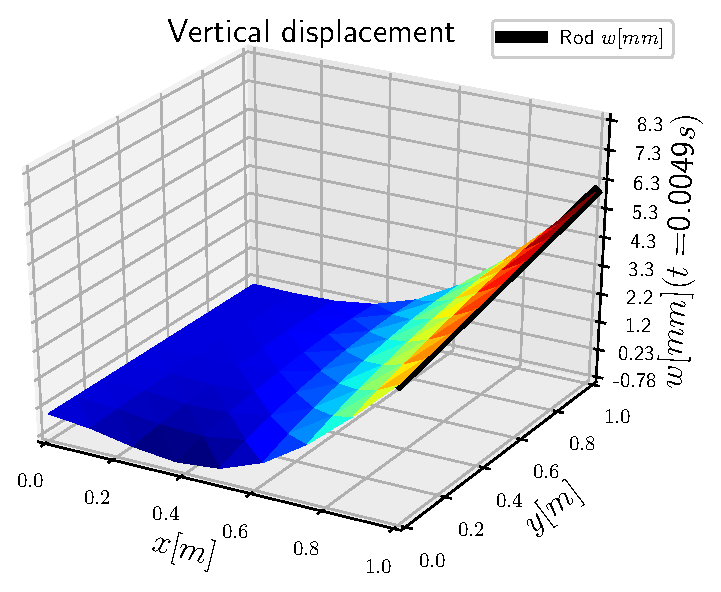
\includegraphics[width=0.25\linewidth]{SnapRod_t50_cropped.eps}%
		\label{fig:Rod_2}}
	\subfloat[$t=0.75 \; t_{\text{end}}$]{\includegraphics[width=0.25\linewidth]{SnapRod_t75_cropped.eps}%
		\label{fig:Rod_3}}
	\hfil
	\subfloat[$t= t_{\text{end}}$]{\includegraphics[width=0.25\linewidth]{SnapRod_t100_cropped.eps}%
		\label{fig:Rod_4}}
	\caption{Snapshots at 4 different times ($t_{\text{end}} = 10 \,[ms]$) of a cantilever plate undergoing solicitation \eqref{eq:force_rod}. The plate is connected to a rigid rod in $x = L_x$. Note the different deformation amplitude with respect to Fig. \ref{fig:IntNoRod}.}
	\label{fig:IntRod}
\end{figure*}
Snapshots of simulations without and with the rigid rod are reported in Figs. \ref{fig:IntNoRod}, \ref{fig:IntRod}\footnote{\label{note:1}Complete videos are accessible at \url{https://github.com/andreabrugnoli/Goodies_pH_plates}}. The deformations undergone by the plate are clearly affected by the presence of the rod: the maximum deformation as well as the Hamiltonian value \ref{fig:HamInt}, once the excitation is removed, are lower. The interconnected side remains straight during the whole simulation, meaning that the constraints are respected.
\section{Boundary control by Damping Injection}
\begin{figure}[t]
	\centering
	\includegraphics[width=0.6\linewidth]{HamiltonianDamped_cropped.eps}
	\caption{Hamiltonian trend considering a boundary control by damping injection.}
	\label{fig:H_Damped}
\end{figure}
\label{sec:Damp}
In \cite{MacchelliMindlin} the damping injection tecnique was used to stabilize the Mindlin plate subjected to an initial condition. Here the stabilization of a cantilever Kirchoff plate is performed. Starting from system \eqref{eq:discr_pl}, consider the following static control law
\begin{equation}
\bm{u} = -\bm{K} \bm{y}.
\end{equation}
System \eqref{eq:discr_pl} now reads
\begin{equation}
\begin{bmatrix}
\bm{M}_{\text{pl}} & \bm{0} \\
\bm{0} & \bm{0} \\
\end{bmatrix}\frac{\d}{\d t}
\begin{pmatrix}
\bm{e}_{\text{pl}}\\
\bm{\lambda}_D \\
\end{pmatrix}
= \begin{bmatrix}
\bm{J}_d - \bm{R} & \bm{G}_D \\
-\bm{G}_D^T & \bm{0} \\
\end{bmatrix}
\begin{pmatrix}
\bm{e}_{\text{pl}}\\
\bm{\lambda}_D \\
\end{pmatrix}.
\end{equation}
The matrix $\bm{R} = \bm{B}_N \bm{Z} \bm{B}_N^T \succcurlyeq 0$ is semi-positive definitive because of the collocated input-output feature of pH systems. The energy rate evaluates to (\cite{beattie2018linear} theorem 13)
\[\dot{H} _{\text{pl}} = - \bm{e}_{\text{pl}}^T \; \bm{R} \; \bm{e}_{\text{pl}} \le 0. \]
Therefore, the Hamiltonian energy is a Lyapunov function and the asymptotic stability of configuration $\bm{e}_{\text{pl}} = \bm{0}$ is deduced using LaSalle' invariance  principle (\cite{bookPHs}  chapter 6, proposition 6.2). As a numerical illustration a cantilever square plate clamped in $x=0$ with parameters given in Table~\ref{tab:par} is considered. The controller gain matrix is set to $\bm{K} = 100 \ \bm{I}$. The initial condition, that must be compatible with the constraints, reads
\[e_w(x,y,0) = x^2, \quad \bm{E}_{\kappa}(x,y,0)=0\]
The control law is activated after 1 second. The discrete Hamiltonian, computed using \eqref{eq:H_discr} goes almost to zero in 4 seconds (Fig. \ref{fig:H_Damped}). Snapshot of simulation, reported in Fig.~\ref{fig:SnapDamp}, show the decreasing amplitudes of the oscillations\footnote{See footnote \ref{note:1}}, as the plate gradually reaches the undeformed equilibrium state.

\begin{figure*}[t]
	\centering
	\subfloat[$t=0.03 \; t_{\text{end}}$]{\includegraphics[width=0.25\linewidth]{Snapshot_t30_cropped.eps}%
		\label{fig:Damp_1}}
	\subfloat[$t=0.06 \; t_{\text{end}}$]{\includegraphics[width=0.25\linewidth]{Snapshot_t60_cropped.eps}%
		\label{fig:Damp_2}}
	\subfloat[$t=0.28 \; t_{\text{end}}$]{\includegraphics[width=0.25\linewidth]{Snapshot_t280_cropped.eps}%
		\label{fig:Damp_3}}
	\subfloat[$t=0.32 \, t_{\text{end}}$]{\includegraphics[width=0.25\linewidth]{Snapshot_t320_cropped.eps}%
		\label{fig:Damp_4}}
		\hfil
		\subfloat[$t=0.475 \; t_{\text{end}}$]{\includegraphics[width=0.25\linewidth]{Snapshot_t475_cropped.eps}%
			\label{fig:Damp_5}}
		\subfloat[$t=0.57 \; t_{\text{end}}$]{\includegraphics[width=0.25\linewidth]{Snapshot_t570_cropped.eps}%
			\label{fig:Damp_6}}
		\subfloat[$t=0.73 \; t_{\text{end}}$]{\includegraphics[width=0.25\linewidth]{Snapshot_t730_cropped.eps}%
			\label{fig:Damp_7}}
		\subfloat[$t=0.965 \, t_{\text{end}}$]{\includegraphics[width=0.25\linewidth]{Snapshot_t965_cropped.eps}%
			\label{fig:Damp_8}}
		\hfil
	\caption{Snapshots at different times of the simulation for the boundary controller by damping injection ($t_{\text{end}} = 5 \,[s]$). The plate is clamped at $x = 0$ and the controller acts on the rest of the boundary $\Gamma_{\text{control}} = \left\{(x,y) \vert\; x=L_x \cup y=0 \cup y = L_y \right\}$.}
	\label{fig:SnapDamp}
	\hfil
\end{figure*}


\section{Conclusion}
In this paper the port-Hamiltonian tensorial formulation has been discussed. A structure preserving discretization is obtained by applying a mixed finite element method. The resulting system explicitly contain the boundary variables, so that the interconnection with other finite or infinite-dimensional systems can be easily performed. As a control application the damping injection methodology was addressed.



%\addtolength{\textheight}{-1.3cm}   % This command serves to balance the column lengths
% on the last page of the document manually. It shortens
% the textheight of the last page by a suitable amount.
% This command does not take effect until the next page
% so it should come on the page before the last. Make
% sure that you do not shorten the textheight too much.



% conference papers do not normally have an appendix


% use section* for acknowledgment
\section*{Acknowledgment}
The authors would like to thank Ghislain Haine, Michel Salau\"n and Xavier Vasseur from ISAE-SUPAERO for their insightful observations and comments.

\bibliographystyle{IEEEtran}
\bibliography{biblio_CDCKirchhoff}

% An example of a floating figure using the graphicx package.
% Note that \label must occur AFTER (or within) \caption.
% For figures, \caption should occur after the \includegraphics.
% Note that IEEEtran v1.7 and later has special internal code that
% is designed to preserve the operation of \label within \caption
% even when the captionsoff option is in effect. However, because
% of issues like this, it may be the safest practice to put all your
% \label just after \caption rather than within \caption{}.
%
% Reminder: the "draftcls" or "draftclsnofoot", not "draft", class
% option should be used if it is desired that the figures are to be
% displayed while in draft mode.
%
%\begin{figure}[!t]
%\centering
%\includegraphics[width=2.5in]{myfigure}
% where an .eps filename suffix will be assumed under latex, 
% and a .pdf suffix will be assumed for pdflatex; or what has been declared
% via \DeclareGraphicsExtensions.
%\caption{Simulation results for the network.}
%\label{fig_sim}
%\end{figure}

% Note that the IEEE typically puts floats only at the top, even when this
% results in a large percentage of a column being occupied by floats.


% An example of a double column floating figure using two subfigures.
% (The subfig.sty package must be loaded for this to work.)
% The subfigure \label commands are set within each subfloat command,
% and the \label for the overall figure must come after \caption.
% \hfil is used as a separator to get equal spacing.
% Watch out that the combined width of all the subfigures on a 
% line do not exceed the text width or a line break will occur.
%
%\begin{figure*}[!t]
%\centering
%\subfloat[Case I]{\includegraphics[width=2.5in]{box}%
%\label{fig_first_case}}
%\hfil
%\subfloat[Case II]{\includegraphics[width=2.5in]{box}%
%\label{fig_second_case}}
%\caption{Simulation results for the network.}
%\label{fig_sim}
%\end{figure*}
%
% Note that often IEEE papers with subfigures do not employ subfigure
% captions (using the optional argument to \subfloat[]), but instead will
% reference/describe all of them (a), (b), etc., within the main caption.
% Be aware that for subfig.sty to generate the (a), (b), etc., subfigure
% labels, the optional argument to \subfloat must be present. If a
% subcaption is not desired, just leave its contents blank,
% e.g., \subfloat[].


% An example of a floating table. Note that, for IEEE style tables, the
% \caption command should come BEFORE the table and, given that table
% captions serve much like titles, are usually capitalized except for words
% such as a, an, and, as, at, but, by, for, in, nor, of, on, or, the, to
% and up, which are usually not capitalized unless they are the first or
% last word of the caption. Table text will default to \footnotesize as
% the IEEE normally uses this smaller font for tables.
% The \label must come after \caption as always.
%
%\begin{table}[!t]
%% increase table row spacing, adjust to taste
%\renewcommand{\arraystretch}{1.3}
% if using array.sty, it might be a good idea to tweak the value of
% \extrarowheight as needed to properly center the text within the cells
%\caption{An Example of a Table}
%\label{table_example}
%\centering
%% Some packages, such as MDW tools, offer better commands for making tables
%% than the plain LaTeX2e tabular which is used here.
%\begin{tabular}{|c||c|}
%\hline
%One & Two\\
%\hline
%Three & Four\\
%\hline
%\end{tabular}
%\end{table}


% Note that the IEEE does not put floats in the very first column
% - or typically anywhere on the first page for that matter. Also,
% in-text middle ("here") positioning is typically not used, but it
% is allowed and encouraged for Computer Society conferences (but
% not Computer Society journals). Most IEEE journals/conferences use
% top floats exclusively. 
% Note that, LaTeX2e, unlike IEEE journals/conferences, places
% footnotes above bottom floats. This can be corrected via the
% \fnbelowfloat command of the stfloats package.

	
	% that's all folks
\end{document}


